%如果你不清楚LaTeX是什么,非常建议你先在b站查看下面这个教程
%https://www.bilibili.com/video/BV11h41127FD/?spm_id_from=333.337.search-card.all.click&vd_source=d6d1d5fb61de1b6aa08d061642ba52f7
%如果你更喜欢阅读文档,可以到https://www.ctan.org/pkg/lshort-zh-cn这个网站阅读入门文档
%文章中的大部分文字内容是用\lipsum命令随机生成的,如果你只想了解怎么添加中文可以跳到\section{Demo Chinese}部分查看
\documentclass{article}
\usepackage{graphicx}
\usepackage[svgnames]{xcolor}
\usepackage{fancyhdr}
\usepackage{tikz}
\usepackage{lipsum}
\usepackage{ifthen}
\usepackage{pgfmath}
\usepackage{amsmath}
\usepackage{listings}
\lstset{
  language=Python,
  basicstyle=\ttfamily,
  keywordstyle=\color{blue},
  stringstyle=\color{purple},
  commentstyle=\color{gray},
  numbers=left,
  numberstyle=\tiny\color{gray},
  frame=single,
  breaklines=true,
  breakatwhitespace=true,
  showstringspaces=false,
  tabsize=2
}
\usepackage{booktabs}
\usepackage[margin=1in, headheight=30pt, bottom=1in]{geometry}
\usepackage{xeCJK}

\setCJKmainfont{SimSun}

\definecolor{ponyPink}{RGB}{226,87,168}
\definecolor{ponyPurple}{RGB}{119,105,165}

\usetikzlibrary{calc}

\pagestyle{fancy}
\fancyhf{}
\fancyhead[L]{\textcolor{ponyPurple}{\sffamily\bfseries My Little Pony Template}} %‘My Little Pony Template’可以替换成自己想要的标题
\renewcommand{\headrulewidth}{0pt}
\begin{document}
\begin{titlepage}
  \centering
  \vspace*{2cm}
  {\fontsize{40}{48}\selectfont \textcolor{ponyPink}{\sffamily\bfseries My Little Pony Template}} %与上面同理,‘My Little Pony Template’可以替换
  \vskip1cm
  {\Large by Your Name}
  \vfill
  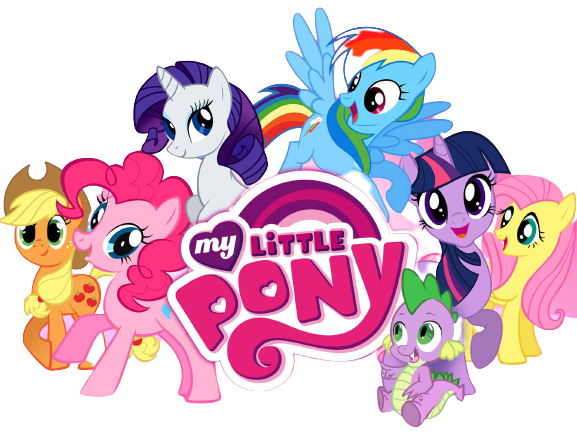
\includegraphics[width=6cm]{my_little_pony_icon5} %如果不喜欢第一页封面图片,可以在网上下载想要的图片到同一目录,将‘my_little_pony_icon5’替换成下载图片的名称
  \vfill
  {\Large May 2023}
\end{titlepage}

\fancyfoot[C]{\thepage}
\fancyfoot[R]{%
  \pgfmathrandominteger{\randompony}{1}{6}
  \includegraphics[width=2cm]{pony\randompony}%
}




\lipsum[1-3] %生成随机文字,可以删除然后书写自己需要的笔记等

%示例如何插入图片,如需插入图片将demo_image改成自己需要的图片名即可,图片应和.tex文件在同一目录下
\section{Demo Image}
\lipsum[4]
\begin{figure}[h]
  \centering
  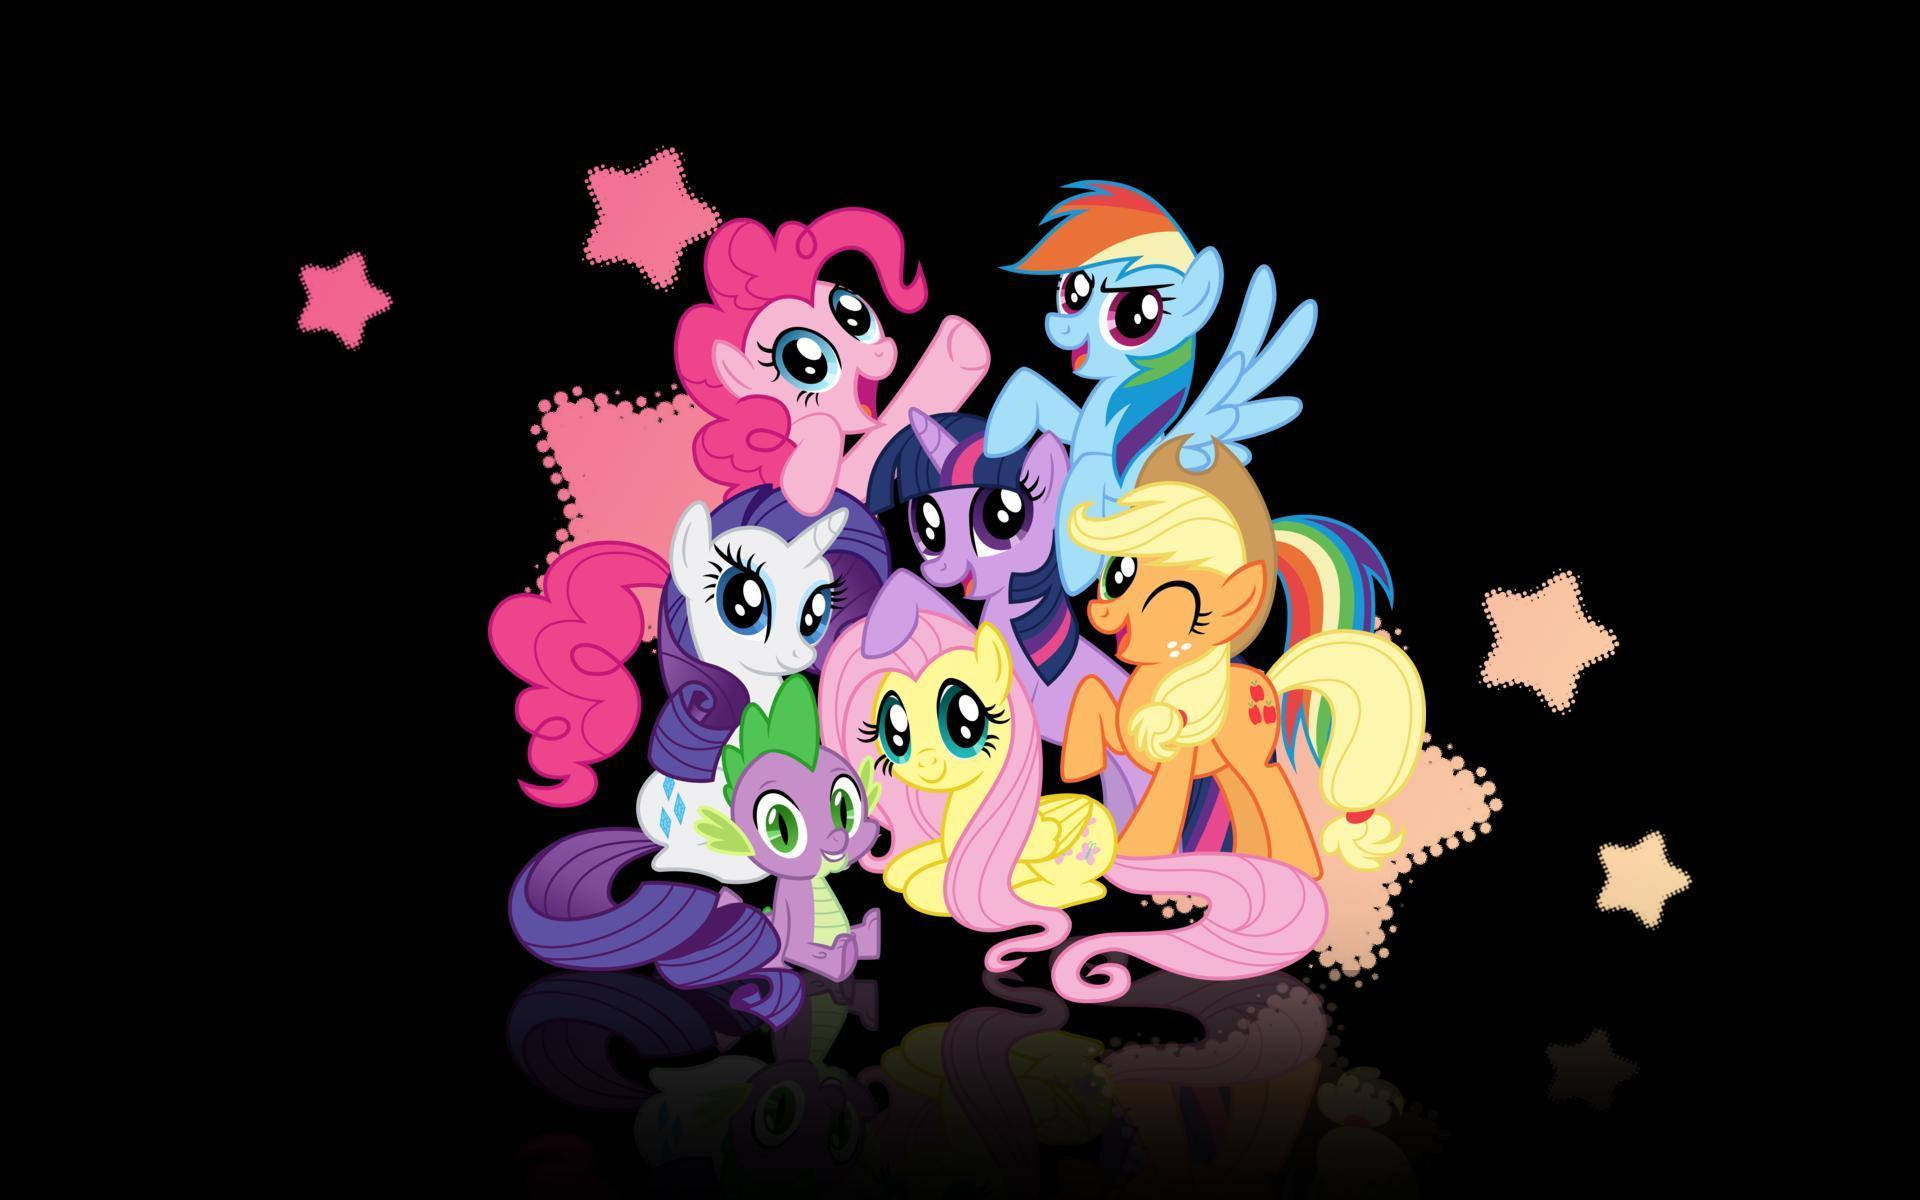
\includegraphics[width=8cm]{demo_image}
  \caption{Demo Image}
  \label{fig:demo-image}
\end{figure}
%示例如何插入数学公式
\section{Mathematical Formulas}
\lipsum[5]
\begin{align*}
  f(x) & = x^2 + 2x + 1         \\
  g(x) & = \frac{1}{\sqrt{x+1}}
\end{align*}
%示例如何插入表格
\section{Table}
\lipsum[6]
\begin{table}[h]
  \centering
  \begin{tabular}{ccc}
    \toprule
    \textbf{Column 1} & \textbf{Column 2} & \textbf{Column 3} \\
    \midrule
    Value 1           & Value 2           & Value 3           \\
    Value 4           & Value 5           & Value 6           \\
    \bottomrule
  \end{tabular}
  \caption{Demo Table}
  \label{tab:demo-table}
\end{table}
%示例如何插入代码
\section{Highlighted Python Code}
\lipsum[7]
\begin{lstlisting}[language=Python, caption=Python Code, label=lst:python-code]
def factorial(n):
    if n == 0:
        return 1
    else:
        return n * factorial(n-1)

num = 5
print("Factorial of", num, "is", factorial(num))
\end{lstlisting}
% \section{Highlighted Python Code}
% \lipsum[7]
% \begin{lstlisting}[caption=Python Code, label=lst:python-code]
% def factorial(n):
% if n == 0:
% return 1
% else:
% return n * factorial(n-1)

% num = 5
% print("Factorial", "of", num, "is", factorial(num))
% \end{lstlisting}

%示例tikz画图
\section{Demo TikZ Picture}
\lipsum[8]
\begin{figure}[h]
  \centering
  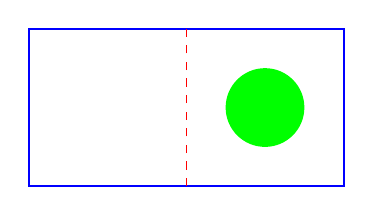
\begin{tikzpicture}
    \draw[blue, thick] (0,0) rectangle (4,2);
    \draw[red, dashed] (2,0) -- (2,2);
    \fill[green] (3,1) circle (0.5);
  \end{tikzpicture}
  \caption{Demo TikZ Picture}
  \label{fig:demo-tikz}
\end{figure}
\section{Demo Chinese}
这是一个中文句子的示例。
我喜欢小马宝莉。
中文也可以很好地显示在 LaTeX 文档中。
《小马宝莉:友情就是魔法》(英语:My Little Pony: Friendship is Magic,台湾译《彩虹小马:友情就是魔法》)是一部基于孩之宝小马宝莉系列玩具与动画作品,
由萝伦·浮士德为孩之宝开发的儿童奇幻动画剧集,常被称之为小马宝莉第四代(“G4”)产品,
由美国有线电视频道The Hub(Discovery Family的前身)于2010年10月10日首播。
该剧起初由萝伦·浮士德担任创意总监与执行制作,她寻求突破小马宝莉系列早已存在的“女孩”本质,
并依循着孩之宝对于“教育与资讯”内涵与玩具系列市场的建议,创造出更深刻的角色与更大胆的设定。
浮士德已于第二季中引退,由监制导演杰森·蒂森接手第二季之后的执行制作。
\section{Random words}
\lipsum[9-40]
\end{document}


